\graphicspath{{./Software/img/}}
\chapter{SignRecognition}
 

\section{Depth Image Processing}
Before trying to do template matching in the camera image, it's necessary to limit the regions in which we are
searching for known templates. Therefore it is necessary to find surfaces which are upright to the camera view.
In beginning the focus almost lies on improving image quality by removing the noise and so it is here.

\subsection{First Blur Filter}
Bluring the depth image to remove the noise sounds like an easy task but if a simple boxed filter is used 
all edges are smothed to surfaces they do not belong to (see first picture in figure \vref{figure:blur}).
At first it was tried to do all the filtering and reset all blured pixels $P_b$ which are to far away from their 
original depth value by the following formula.

\[
 \forall P_b(x,y)  |   \left(\left|{P_b(x,y)-P(x,y)}\right|>{\frac{P(x,y)^2}{480000}}\right)\implies P_b(x,y)=P(x,y)
\]

The following listing \vref{lst:fstBlur} shows the code of this first filter, which uses a box-filter and and a 
median-blur filter from OpenCV. In the next step the previous formula is used to revert pixels and 
then another blur filter is applied to remove possible noise resulting from that procedure 
(see figure \vref{figure:blur} for results).

\newpage

\begin{lstlisting}[caption={Code of the first Bluring Function}\label{lst:fstBlur},language=c++]
void myFilter1(const cv::Mat &src, cv::Mat &dst)
{
	cv::Mat filter_in = src.clone();
	cv::Mat filter=filter_in.clone();
	cv::boxFilter(filter, filter, 3, cv::Size(7, 3), cv::Point(-1, -1), 1, 0);
	cv::medianBlur(filter, filter, 3);
	
	//Update non zero pixels
	for (int y = 0; y < src.rows; y++)
	{
		for (int x = 0; x < src.cols; x++)
		{
			short realValue = filter_in.at<Vec1shrt>(y, x)[0];
			short filteredValue = filter.at<Vec1shrt>(y, x)[0];
			short maxDifference = pow((float)realValue, 2) / (480000);
			if (realValue>0)
			{
				if(abs(realValue - filteredValue) > maxDifference)
				{
					dst.at<Vec1shrt>(y, x)[0] = realValue;
				}
				else
				{
					dst.at<Vec1shrt>(y, x)[0] = filteredValue;
				}
			}
		}
	}
	cv::medianBlur(dst, dst, 3);
}
\end{lstlisting}

\begin{figure}[htp]
\begin{center}
  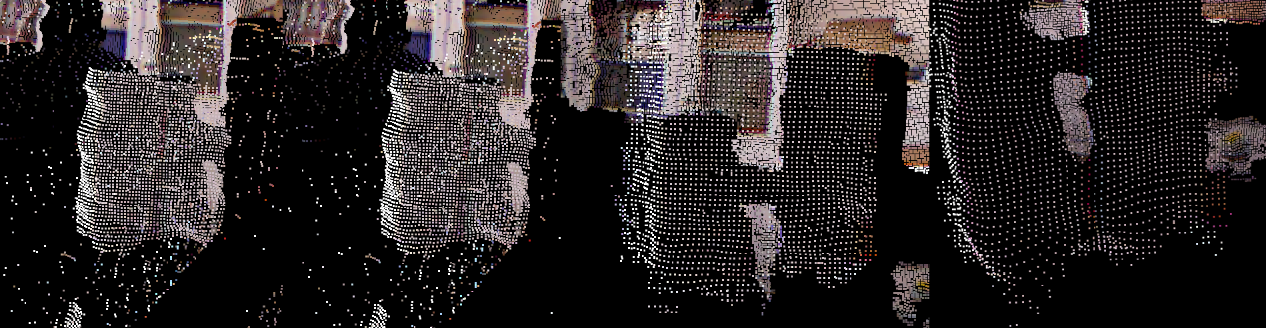
\includegraphics[width=\textwidth]{myFilter1.png}
  \caption{Blur Filter (Boxed/Median/Reset Borders/Median)}
  \label{figure:blur}
\end{center}
\end{figure}
\clearpage

\subsection{Neighborhood Map and New Blur Filter} \label{sect:blurFilter} 
After realizing that there are only 824 depth values available, it was decided to transform the depth picture
to the available depth steps. The resulting step map contains the number of each available depth like 
shown in figure \vref{figure:stepMap}. The converting function uses an array. This array contains the number of the
step when obtaining the cell number of its value. Each cell of a non-existing value contains -1, so it is
possible to check if something is wrong with the value and if it might be not an Kinect RAW picture. 

\begin{figure}[htp]
\begin{center}
  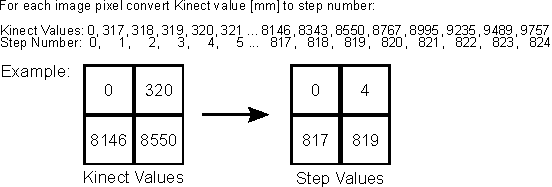
\includegraphics[width=\textwidth]{stepmap.pdf}
  \caption{Step Map Creation}
  \label{figure:stepMap}
\end{center}
\end{figure}

Listing \vref{lst:stpmap} contains the code of the converting function.

\begin{lstlisting}[caption={covertKinectRawToSteps - Function}\label{lst:stpmap}, language=c++]
void convertKinectRawToSteps(const cv::Mat &src, cv::Mat &dst)
{
	if(src.type() == CV_16UC1)
	{
		dst=src.clone();

		int size_x=src.cols, size_y=src.rows;

		for (int i = 0; i < (size_x*size_y); i++)
		{
			//Forward direction x -
			int y_xfw=i/size_x, x_xfw=i-y_xfw*size_x;
			short current=src.at<Vec1shrt>(y_xfw,x_xfw)[0];
			if(current>=0 && current < kinect_depths_count)
			{
				if(kinect_depth_to_step_LUT[current]>=0)
				{
					dst.at<Vec1shrt>(y_xfw,x_xfw)[0]=kinect_depth_to_step_LUT[current];
				}
				else
				{
					std::cerr<<"convertKinectRawToSteps: Unregistered Depth Value found!" 
					           " You must use unedited KINECT RAW data for this! "
							 <<"Value is: "<<current<<std::endl;
				}
			}
			else
			{
				std::cerr<<"convertKinectRawToSteps: Unregistered Depth Value found " 
				           "(too big)! You must use unedited KINECT RAW data for this! "
						 <<"Value is: "<<current<<std::endl;
			}
		}
	}
	else
	{
		std::cerr<<"convertKinectRawToSteps: Wrong matrix type! "
		"You must use unedited KINECT RAW (CV_16UC1) data for this! "<<std::endl;
	}
}
\end{lstlisting}



With that new image it's now possible to determine if a pixel is a direct neighbor to another one. This is mostly the case,
when the value from the difference of the steps is smaller than or equal to one. A threshold of four is adequate to be sure 
to eliminate the noise created by the fractals which can create a step difference of up to 3 inside a surface. 
So the neighborhood condition of one pixel $P$ to another pixel $P_i$ can be determind by the following formula.

\[
 \forall P_i(x_i,y_i)  |\mbox{   }
 \Big(\left|P_i(x_i,y_i)-P(x,y)\right|<4 \Big) \wedge  P_i(x_i,y_i) \neq 0 %\wedge  P(x,y) \neq 0 
\]
\[
 \implies P_i(x_i,y_i) \mbox{ is a close neighbor to } P(x,y)
\]

With this formula a neighborhood map is created which contains 8-bit values for each pixel, where each bit shows the neighborhood 
condition to one of the eight pixels around the current one (as seen in figure \vref{figure:neighborhoodmap}).

Listing \vref{lst:nbhmap} contains the function which generates the neighborhood map.

\begin{lstlisting}[caption={createRelationNeighbourhoodMap - Function}\label{lst:nbhmap}, language=c++]
void createRelationNeighbourhoodMap(const cv::Mat &src, 
                                    cv::Mat &map_out, 
                                    unsigned short threshold)
{
	cv::Mat in=src.clone();
	map_out=cv::Mat::zeros(src.rows,src.cols,CV_8UC3);

	int size_x=in.cols, size_y=in.rows;

	for (int i = 0; i < (size_x*size_y); i++)
	{
		//Forward direction x
		int y_xfw=i/size_x, x_xfw=i-y_xfw*size_x;

		int x=x_xfw;
		int y=y_xfw;

		int curValue=in.at<Vec1shrt>(y,x)[0];


		bool _IsNotTopRow=(y>0);
		bool _IsNotLeftCol=(x>0);
		bool _IsNotBottomRow=(y<(size_y-1));
		bool _IsNotRightCol=(x<(size_x-1));

		short cnt=0;
		unsigned char neighbors_close=0;
		unsigned char neighbors_nNAN=0;

		if(curValue>0)
		{

			//Top Row
			if(_IsNotTopRow)
			{
				//Left Top Cell
				if(_IsNotLeftCol)
				{
					int C_TL=in.at<Vec1shrt>(y_xfw-1,x_xfw-1)[0]; 
					if(C_TL>0)
					{
						neighbors_nNAN|=0x01;
						if(abs(C_TL-curValue)<threshold) 
						//Bigger then zero and difference to current pixel smaller threshold?
						{
							neighbors_close|=0x01;
							cnt++;
						}
					}
				}

				//Middle Top Cell
				int C_TM=in.at<Vec1shrt>(y_xfw-1,x_xfw)[0];
				if(C_TM>0)
				{
					neighbors_nNAN|=0x02;
					if(abs(C_TM-curValue)<threshold)
					{
						neighbors_close|=0x02;
						cnt++;
					}
				}

				//Right Top Cell
				if(_IsNotRightCol)
				{
					int C_TR=in.at<Vec1shrt>(y_xfw-1,x_xfw+1)[0];
					if(C_TR>0)
					{
						neighbors_nNAN|=0x04;
						if(abs(C_TR-curValue)<threshold)
						{
							neighbors_close|=0x04;
							cnt++;
						}
					}
				}
			}


			//Middle Row

			//Left Middle Cell
			if(_IsNotLeftCol)
			{
				int C_ML=in.at<Vec1shrt>(y_xfw,x_xfw-1)[0];
				if(C_ML>0)
				{
					neighbors_nNAN|=0x80;
					if(abs(C_ML-curValue)<threshold)
					{
						neighbors_close|=0x80;
						cnt++;
					}
				}
			}

			//Right Middle Cell
			if(_IsNotRightCol)
			{
				int C_MR=in.at<Vec1shrt>(y_xfw,x_xfw+1)[0];
				if(C_MR>0)
				{
					neighbors_nNAN|=0x08;
					if(abs(C_MR-curValue)<threshold)
					{
						neighbors_close|=0x08;
						cnt++;
					}
				}
			}

			//Bottom Row
			if(_IsNotBottomRow)
			{
				//Left Bottom Cell
				if(_IsNotLeftCol)
				{
					int C_BL=in.at<Vec1shrt>(y_xfw+1,x_xfw-1)[0];
					if(C_BL>0)
					{
						neighbors_nNAN|=0x40;
						if(abs(C_BL-curValue)<threshold)
						{
							neighbors_close|=0x40;
							cnt++;
						}
					}
				}

				//Middle Bottom Cell
				int C_BM=in.at<Vec1shrt>(y_xfw+1,x_xfw)[0];
				if(C_BM>0)
				{
					neighbors_nNAN|=0x20;
					if(abs(C_BM-curValue)<threshold)
					{
						neighbors_close|=0x20;
						cnt++;
					}
				}

				//Right Bottom Cell
				if(_IsNotRightCol)
				{
					int C_BR=in.at<Vec1shrt>(y_xfw+1,x_xfw+1)[0];
					if(C_BR>0)
					{
						neighbors_nNAN|=0x10;
						if(abs(C_BR-curValue)<threshold)
						{
							neighbors_close|=0x10;
							cnt++;
						}
					}
				}

			}

		}//IF NOT NULL END

		map_out.at<Vec3uchar>(y,x)[0]=neighbors_close;
		map_out.at<Vec3uchar>(y,x)[1]=neighbors_nNAN;
		map_out.at<Vec3uchar>(y,x)[2]=cnt;

	}//FOR END
}
\end{lstlisting}


\begin{figure}[htp]
\begin{center}
  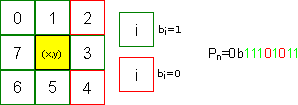
\includegraphics[width=\textwidth]{neighborhoodmap.pdf}
  \caption{Neighborhood-Map Creation}
  \label{figure:neighborhoodmap}
\end{center}
\end{figure}

This information helps to write a more performance saving, effective and edge saving bluring method which 
was named crossBlur because it blures each pixel with a specified number of it's neighbors on top, left, right and bottom.
The neighborhood condition is needed because it will stop adding pixels on each side if the next pixel in the direction 
is not a close neighbor to the current to preserve the edges. (see in figure \vref{figure:crossblur}).

\begin{figure}[htp]
\begin{center}
  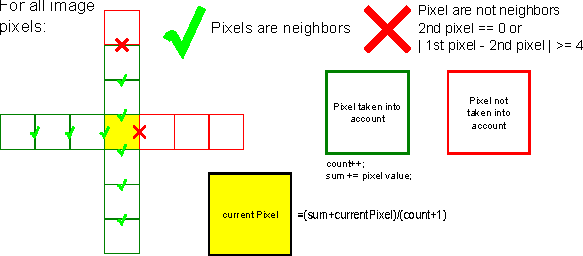
\includegraphics[width=\textwidth]{crossBlur.pdf}
  \caption{Cross Blur Working Principle}
  \label{figure:crossblur}
\end{center}
\end{figure} 

%TODO Formula
%TODO Result picture

Listing \vref{lst:crossblur} shows the cross bluring function.

\begin{lstlisting}[caption={crossDepthBlur - Function}\label{lst:crossblur}, language=c++]
void crossDepthBlur(const cv::Mat &depth, const cv::Mat &neighbors, 
                    cv::Mat &depth_out, int max_size)
{
	cv::Mat dst=cv::Mat::zeros(depth.rows,depth.cols,CV_16UC1);
	int size_x=depth.cols, size_y=depth.rows;
	int y,x;
	for (int i = 0; i < (size_x*size_y); i++)
	{
		y=i/size_x;
		x=i-y*size_x;

		//Sum all pixels
		int sum=depth.at<Vec1shrt>(y, x)[0];

		//If current pixel is 0 go to next
		if(sum == 0) continue;

		//Count all values
		int cnt=1;

		//Get the neighbors of the current pixel
		uchar cur_nb=neighbors.at<Vec3uchar>(y,x)[0];

		//Usable neighbors
		bool nb_top=(1<<1)&cur_nb;
		bool nb_right=(1<<3)&cur_nb;
		bool nb_bottom=(1<<5)&cur_nb;
		bool nb_left=(1<<7)&cur_nb;

		for(int j=1; j<=max_size; j++)
		{
			if(nb_top)
			{
				nb_top=neighbors.at<Vec3uchar>(y-j,x)[0]&(1<<1);
				sum+=depth.at<Vec1shrt>(y-j, x)[0];
				cnt++;
			}
			if(nb_right)
			{
				nb_right=neighbors.at<Vec3uchar>(y,x+j)[0]&(1<<3);
				sum+=depth.at<Vec1shrt>(y, x+j)[0];
				cnt++;
			}
			if(nb_bottom)
			{
				nb_bottom=neighbors.at<Vec3uchar>(y+j,x)[0]&(1<<5);
				sum+=depth.at<Vec1shrt>(y+j, x)[0];
				cnt++;
			}
			if(nb_left)
			{
				nb_left=neighbors.at<Vec3uchar>(y,x-j)[0]&(1<<7);
				sum+=depth.at<Vec1shrt>(y, x-j)[0];
				cnt++;
			}

			//If no suitable neighbor is available exit loop
			if(nb_left + nb_right + nb_top + nb_bottom == 0) break;
		}

		dst.at<Vec1shrt>(y,x)=sum/cnt;
	}
	depth_out=dst;
}
\end{lstlisting}

\subsection{Calculation of X and Y Distance}
After bluring the depth the real world X and Y values of each point must be calculated. 
This is done with the camera information delivered from ROS. 
The code for this is mostly copied from the rgbxyz-point cloud nodelet from ROS with a few changes.
All of the float values are multiplied by 100 and converted to integer. This is used to increase the accuracy while
calculating a integer value for x and y coordinates. The coordinates itself are stored as short. This was done to save
computational time by calculating the normals with short instead of the double format.

The full code of the function to create the XY-map is shown in the listing \vref{lst:xymap}.
\begin{lstlisting}[caption={createXYMap - Function\label{lst:xymap}},language=C++]
void createXYMap(const cv::Mat &src, 
				 const sensor_msgs::CameraInfoConstPtr& info_msg, 
				 cv::Mat &xy)
{
	if(src.type() == CV_16UC1)
	{
		xy=cv::Mat::zeros(src.rows,src.cols,CV_16UC2);

		image_geometry::PinholeCameraModel model;
		model.fromCameraInfo(info_msg);

		int center_x = model.cx()*100;	
		int center_y = model.cy()*100;

		int constant_x = model.fx()*100;
		int constant_y = model.fy()*100;

		int size_x=src.cols, size_y=src.rows;

		int x,y;
		for (int i = 0; i < (size_x*size_y); i++)
		{
			y=i/size_x;
			x=i-y*size_x;

			if(x>0)
			{
				short depth=src.at<Vec1shrt>(y,x)[0];
				xy.at<Vec2shrt>(y,x)[0] = ((x*100 - center_x) * depth) / constant_x;
				xy.at<Vec2shrt>(y,x)[1] = ((y*100 - center_y) * depth) / constant_y;
			}
		}
	}
	else
	{
		ROS_ERROR("WRONG TYPE: createXYMap");
	}
}
\end{lstlisting}


\subsection{3D RangeFilter}
If the real X and Y values for each pixel $P_i$ are known, it is possible to get only the pixels $P_o$ for a 
3-dimensional region of interest by setting minimum and maximum values for all axis and removing them from 
the depth image.

	$$
		\forall P_i(x,y) | (X_i < Xmin \vee X_i > Xmax \vee Y_i > Ymax \vee Y_i < Ymin \vee Z_i < Zmin \vee Z_i > Zmax)
	$$$$
		\implies P_o(x,y) = 0;
	$$

Listing \vref{lst:range3d} shows the code of the 3D Range Filter and figure \vref{figure:xyzrange} the working principle.

\begin{lstlisting}[caption={XYZrangeFilter - Function\label{lst:range3d}},language=C++]
void XYZrangeFilter(const cv::Mat &depth, 
                    const cv::Mat &xy, 
                    cv::Mat &depth_out, 
                    int min_x, int max_x, 
                    int min_y, int max_y, 
                    int min_z, int max_z)
{

	int size_x=depth.cols, size_y=depth.rows;
	depth_out=depth.clone();
	int y,x;
	for (int i = 0; i < (size_x*size_y); i++)
	{
		y=i/size_x;
		x=i-y*size_x;


		short cur_z=depth_out.at<Vec1shrt>(y,x)[0];


		if(cur_z == 0) continue; //If depth == 0 continue with next pixel

		int cur_x=xy.at<Vec2shrt>(y,x)[0];
		int cur_y=xy.at<Vec2shrt>(y,x)[1];

		if(!((cur_x >= min_x && cur_x <= max_x)&&
		     (cur_y >= min_y && cur_y <= max_y)&&
		     (cur_z >= min_z && cur_z <= max_z)))
		{
			depth_out.at<Vec1shrt>(y,x)[0]=0;
		}
	}
}
\end{lstlisting}


%\usepackage{graphics} is needed for \includegraphics
\begin{figure}[htp]
\begin{center}
  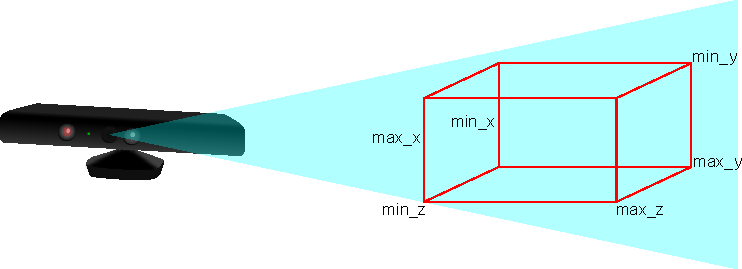
\includegraphics[width=\textwidth]{XYZFilter.pdf}
  \caption{XYZ-Range-Filter Concept}
  \label{figure:xyzrange}
\end{center}
\end{figure}


\subsection{Normal Calculation}
With the depth image and the xy map the normal of each pixel can be calculated. This is done with the scalar product.


$$ \vec{N} = \left( \begin{array}{c} x_u \\ y_u \\ z_u \end{array} \right) \times \left( \begin{array}{c} x_v \\ y_v \\ z_v \end{array} \right) 
= \left( \begin{array}{c} y_u \cdot z_v - z_u \cdot y_v \\ z_u \cdot x_v - z_v \cdot x_u \\ x_u \cdot y_v - y_u \cdot x_v \end{array}\right)
$$

The current algorithm tries to calculate two normals, one calculated with the vector from the current pixel to the top and right 
($\vec{N_{tr}}=\vec{V_t}\times\vec{V_r}$) and one to
the bottom and left ($\vec{N_{bl}}=\vec{V_b}\times\vec{V_l}$). 
If both normals can be calculated it takes the average of both normals (see figure \vref{figure:normals}).

$$ \vec{N} = \frac{\vec{N_{tr}} + \vec{N_{bl}}}{2}$$

\begin{figure}[htp]
\begin{center}
  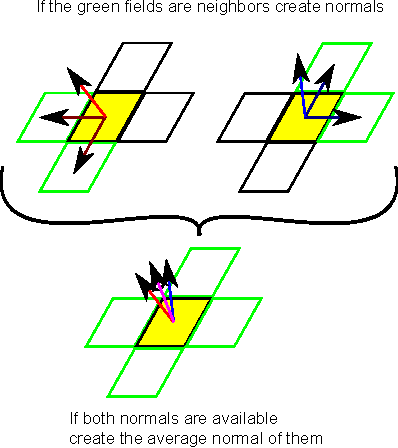
\includegraphics[width=\textwidth/3]{normals.pdf}
  \caption{Normals Creation}
  \label{figure:normals}
\end{center}
\end{figure}

\subsection{Angle Calculation}

The angles from vectors to the axes are basically calculated by the follwing formulas. Where $\alpha$, $\beta$ and $\gamma$ 
are the angles to the x,y, and z-axis of the normal vector $\vec{N}$ as seen in figure \vref{figure:NormalAngles}.

\begin{figure}[htp]
\begin{center}
  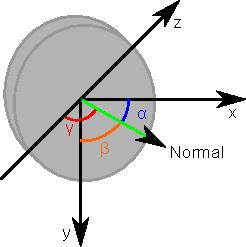
\includegraphics[width=\textwidth/3]{Angles.pdf}
  \caption{Angles of a Normal}
  \label{figure:NormalAngles}
\end{center} 
\end{figure}

$$ \alpha = \arccos \frac{N_x}{\left|\vec{N}\right|}  $$
$$ \beta  = \arccos \frac{N_y}{\left|\vec{N}\right|}  $$
$$ \gamma = \arccos \frac{N_z}{\left|\vec{N}\right|}  $$

In the application the arcus cosinus values are precalculated to save computational time.
The possible input range for the arcus cosinus function lies between -1 and 1, so it was decided
to precalculate 2000 values for the lookup table. This means the possible input values are now
-1000 to 1000. To bring them into the possible range 1000 needs to be added to all input values.
The precalulated values also include the transformation from radian to degree and are stored as 
integers values which were multiplied by 100 to save two digits behind the comma.

So the precalculation for the values $v_i$ in the array was done with the following formula:

$v_i=\lfloor \arccos ((i-1000)/1000) * \frac{180}{\pi}*100 + 0,5 \rfloor$

To obtain the values from the array the result of the devision from a vector part through its length
must be multiplied with 1000 and added to 1000. To be able to display the angles easily for debuging 
it was later decided to put the values in a matrix for an RGB image, so each value has to be devided 
by 100 again because unsigned char only supports values from 0 to 255.

The following listing \vref{lst:AngleMap} shows the code for the angle calculation function.

\begin{lstlisting}[caption={createAngleMap - Function}\label{lst:AngleMap},language=c++]
void createAngleMap(const cv::Mat &normals, cv::Mat &angles)
{
	angles=cv::Mat::zeros(normals.rows,normals.cols,CV_8UC3);
	int size_x=normals.cols, size_y=normals.rows;
	int y,x;
	for (int i = 0; i < (size_x*size_y); i++)
	{ 
		y=i/size_x;
		x=i-y*size_x;

		short g1=(normals.at<Vec3shrt>(y,x)[0]);
		short g2=(normals.at<Vec3shrt>(y,x)[1]);
		short g3=(normals.at<Vec3shrt>(y,x)[2]);

		double vector_length=sqrt(g1*g1+g2*g2+g3*g3);
		if(!vector_length)continue;

		angles.at<Vec3uchar>(y,x)[0]=preCalcCos[(int)(g1*1000/vector_length)+1000]/100;
		angles.at<Vec3uchar>(y,x)[1]=preCalcCos[(int)(g2*1000/vector_length)+1000]/100;
		angles.at<Vec3uchar>(y,x)[2]=preCalcCos[(int)(g3*1000/vector_length)+1000]/100;
	}
}	
\end{lstlisting}

\subsection{Angle Bluring}

To blur the angles the same method as mentioned in chapter \vref{sect:blurFilter} was used and
the average was done for each angle seperately. The comparison between a blured and a non-blured
angle picture is shown in figure \vref{figure:AnglesBlured}.

\begin{figure}[htp]
\begin{center}
  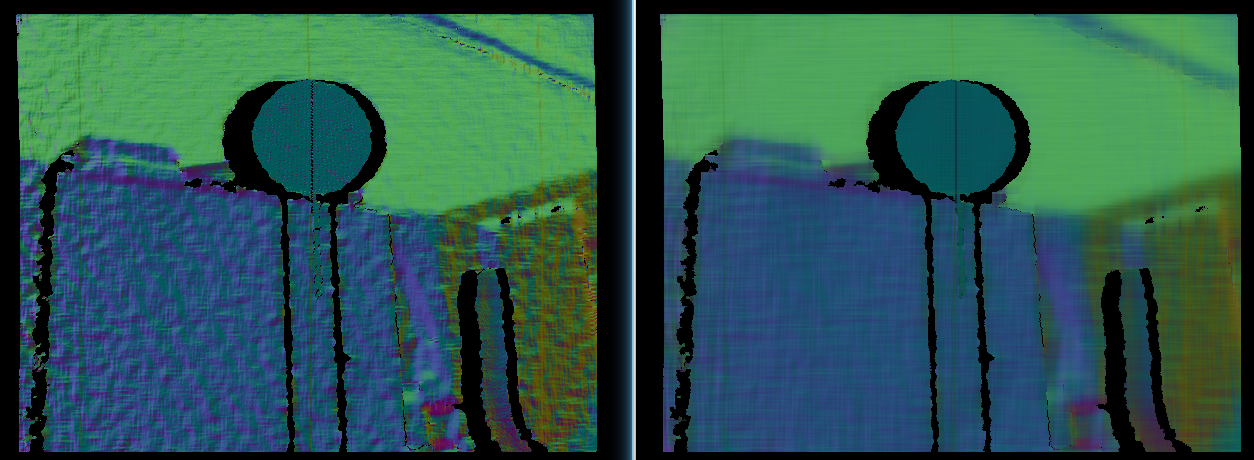
\includegraphics[width=\textwidth]{AnglesMapBlured.png}
  \caption{Angles Map non-blured and blured}
  \label{figure:AnglesBlured}
\end{center}
\end{figure}




Listing \vref{lst:AngleBlur} contains the source for the angle bluring function.

\begin{lstlisting}[caption={crossAnglesBlur - Function}\label{lst:AngleBlur},language=c++]
void crossAnglesBlur(const cv::Mat &angles, 
                     const cv::Mat &neighbors, 
                     cv::Mat &angles_out, int max_size)
{

	cv::Mat dst=cv::Mat::zeros(angles.rows,angles.cols,CV_8UC3);
	int size_x=angles.cols, size_y=angles.rows;
	int y,x;
	for (int i = 0; i < (size_x*size_y); i++)
	{
		y=i/size_x;
		x=i-y*size_x;

		//Get the neighbors of the current pixel
		uchar cur_nb=neighbors.at<Vec3uchar>(y,x)[0];
		if(cur_nb == 0) continue;


		//Sum all pixels
		int sum_x=angles.at<Vec3uchar>(y, x)[0];
		int sum_y=angles.at<Vec3uchar>(y, x)[1];
		int sum_z=angles.at<Vec3uchar>(y, x)[2];

		//Count all values
		int cnt=1;

		//Usable neighbors
		bool nb_top=(1<<1)&cur_nb;
		bool nb_right=(1<<3)&cur_nb;
		bool nb_bottom=(1<<5)&cur_nb;
		bool nb_left=(1<<7)&cur_nb;

		for(int j=1; j<=max_size; j++)
		{
			if(nb_top)
			{
				nb_top=neighbors.at<Vec3uchar>(y-j,x)[0]&(1<<1);
				sum_x+=angles.at<Vec3uchar>(y-j, x)[0];
				sum_y+=angles.at<Vec3uchar>(y-j, x)[1];
				sum_z+=angles.at<Vec3uchar>(y-j, x)[2];
				cnt++;
			}
			if(nb_right)
			{
				nb_right=neighbors.at<Vec3uchar>(y,x+j)[0]&(1<<3);
				sum_x+=angles.at<Vec3uchar>(y, x+j)[0];
				sum_y+=angles.at<Vec3uchar>(y, x+j)[1];
				sum_z+=angles.at<Vec3uchar>(y, x+j)[2];
				cnt++;
			}
			if(nb_bottom)
			{
				nb_bottom=neighbors.at<Vec3uchar>(y+j,x)[0]&(1<<5);
				sum_x+=angles.at<Vec3uchar>(y+j, x)[0];
				sum_y+=angles.at<Vec3uchar>(y+j, x)[1];
				sum_z+=angles.at<Vec3uchar>(y+j, x)[2];
				cnt++;
			}
			if(nb_left)
			{
				nb_left=neighbors.at<Vec3uchar>(y,x-j)[0]&(1<<7);
				sum_x+=angles.at<Vec3uchar>(y, x-j)[0];
				sum_y+=angles.at<Vec3uchar>(y, x-j)[1];
				sum_z+=angles.at<Vec3uchar>(y, x-j)[2];
				cnt++;
			}

			//If no suitable neighbor is available exit loop
			if(nb_left + nb_right + nb_top + nb_bottom == 0) break;
		}

		dst.at<Vec3uchar>(y,x)[0]=sum_x/cnt;
		dst.at<Vec3uchar>(y,x)[1]=sum_y/cnt;
		dst.at<Vec3uchar>(y,x)[2]=sum_z/cnt;
	}
	angles_out=dst;
}
\end{lstlisting}

\subsection{Angle Filtering}

To get only surfaces which are interesting a angle filter was created. It's input parameters
are the minimum and maxium for each angle. The output of this function is a grascale image
where pixels all $P_o$ are initialized with 0 and those with suitable angles 
for the input pixel $P_i$ get the value 255.

 \[
 	\forall P_i(x,y) | (\alpha_i<=max\_\alpha \wedge \alpha_i>=min\_\alpha) \wedge
 	(\beta_i<=max\_\beta \wedge \beta_i>=min\_\beta) \]\[ \wedge (\gamma_i<=max\_\gamma \wedge \gamma_i>=min\_\gamma)
 \]\[
 	\implies P_o(x,y) = 255;
 \] 

The function also features another mode where the output image contains the suitable angles instead of only 255.
But this mode is not used. The full code of this, can be seen in the listing \vref{lst:angleFilter}.

\begin{lstlisting}[caption={anglesFilter - Function}\label{lst:angleFilter},language=c++]
void anglesFilter(const cv::Mat &angles, cv::Mat &angles_out, 
                  unsigned int x_angle_min,unsigned int x_angle_max,
                  unsigned int y_angle_min,unsigned int y_angle_max,
                  unsigned int z_angle_min,unsigned int z_angle_max, 
                  bool binary)
{
	cv::Mat dst;
	if(!binary)
	{
		dst=cv::Mat::zeros(angles.rows,angles.cols,CV_8UC3);
	}
	else
	{
		dst=cv::Mat::zeros(angles.rows,angles.cols,CV_8UC1);
	}

	int size_x=angles.cols, size_y=angles.rows;
	int y,x;
	for (int i = 0; i < (size_x*size_y); i++)
	{
		y=i/size_x;
		x=i-y*size_x;
		unsigned int a_x=angles.at<Vec3uchar>(y,x)[0];
		unsigned int a_y=angles.at<Vec3uchar>(y,x)[1];
		unsigned int a_z=angles.at<Vec3uchar>(y,x)[2];

		if(a_x >= x_angle_min && a_x <= x_angle_max && 
	 	   a_y >= y_angle_min && a_y <= y_angle_max && 
	 	   a_z >= z_angle_min && a_z <= z_angle_max )
		{
			if(!binary)
			{
				dst.at<Vec3uchar>(y,x)[0]=a_x;
				dst.at<Vec3uchar>(y,x)[1]=a_y;
				dst.at<Vec3uchar>(y,x)[2]=a_z;
			}
			else
			{
				dst.at<Vec1uchar>(y,x)[0]=255;
			}
		}
	}
	angles_out=dst;
}
\end{lstlisting}



\subsection{Surface Segmentation}

Before the begining with segmenting the surfaces the picture containing the pixels which show correct angles
is blured to remove empty pixels or columns of empty pixels which seperate surfaces belonging together. After
bluring them, the threshold function is used to bring all pixel which are not zero to the value 255. 
The code is shown in listing \vref{lst:blurAthres}.

\begin{lstlisting}[caption={Bluring and Thresholding}\label{lst:blurAthres},language=c++]
	cv::blur(angles_ok,angles_ok,cv::Size(5,5),cv::Point(-1,-1),0);
	cv::threshold(angles_ok,angles_ok,1,255,0);
\end{lstlisting}

The segmentation algorithm uses a class named range to outline pixel blobs in regions. The class contains integer 
variables for the minimal and maximal x and y values. The algorithm seeks for an pixel in the 
neighborhood-map which are not zero, as shown in the chapter \vref{sect:blurFilter}, this means it has neighbors. 

Then it starts to look if there is neighbor with the following order for the pixels, top, top-left, left and bottom-left.
If it finds a pixel which is a neighbor then it gathers it's ID in the IDs matrix, sets the current pixel in the
id matrix to this ID and calls the update function of the corresponding range object, which updates minimum and
maximum values. After that it checks if the rest of the pixels not checked in step one. If it finds a neighbor
which has a different ID, it creates a relation between them inside a set, a special form of vector which allows
only unique items. If this is done for each of the remaining neighbors, the algorithm advances to the next pixel. 
If a pixel contains neighbors, but doesn,t have a neighbor at the mentioned locations a new ID and range object are 
created. The range objects minimum and maximum x and y are initialized to the values of the current pixel.
This part of the algorithm is visualized in figure \vref{figure:segment} and the corresponding code is shown in listing
\vref{lst:SFextract1}.

\begin{figure}[htp]
\begin{center}
  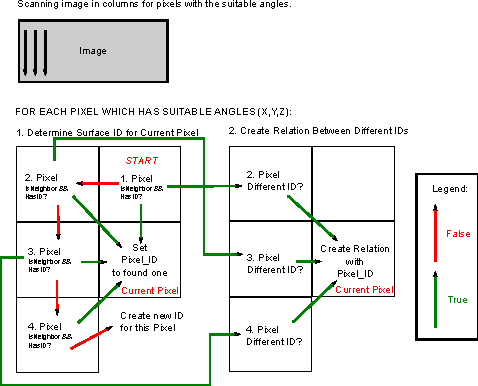
\includegraphics[width=\textwidth]{SurfaceSegmentation.pdf}
  \caption{Segmentation Part 1}
  \label{figure:segment}
\end{center}
\end{figure}

\begin{lstlisting}[caption={SurfaceExtractor - Function Part 1}\label{lst:SFextract1},language=c++]
void SurfaceExtractor(const cv::Mat &pix_ok, 
					  const cv::Mat &neighbors, 
					  std::vector<Match_Roi> &rois, 
					  int minWidth, int minHeight, 
					  int maxWidth, int maxHeight)
{

	cv::Mat ids=cv::Mat::zeros(pix_ok.rows,pix_ok.cols,CV_32SC1);
	int last_id=0;
	std::set< std::pair<int,int> > relations;
	std::vector< Range* > ranges;
	std::vector< Range* > del_ranges;

	int size_x=pix_ok.cols, size_y=pix_ok.rows;
	int y,x;
	for (int i = 0; i < (size_x*size_y); i++)
	{
		//Move forward in vertical direction
		x=i/size_y;
		y=i-x*size_y;

		int current_id=0;
		uchar cur_neighbors=neighbors.at<Vec3uchar>(y,x)[0];
		uchar cur_ok=pix_ok.at<Vec1uchar>(y,x)[0];
		bool found=false;

		if(cur_ok) //current pixel has neighbors and is ok (angle)...
		{
			int id_of_neighbor=0;
			for(int j=0;j<4;j++)
			{
				int neighbor_present, y_n,x_n; //Values for neighbor
				//which neighbor
				switch(j)
				{
				case 0:
					neighbor_present=cur_neighbors&(1<<1); //top
					x_n=x;
					y_n=y-1;
					break;
				case 1:
					neighbor_present=cur_neighbors&(1<<0);	//top-left
					x_n=x-1;
					y_n=y-1;
					break;
				case 2:
					neighbor_present=cur_neighbors&(1<<7); //left
					x_n=x-1;
					y_n=y;
					break;
				case 3:
					neighbor_present=cur_neighbors&(1<<6); //bottom-left
					x_n=x-1;
					y_n=y+1;
					break;
				}

				if(neighbor_present)
				{
				    //look if there is already an ID
					id_of_neighbor=ids.at<Vec1int>(y_n,x_n)[0]; 

					//if there is one and no ID was found before
					if(id_of_neighbor>0 && !found) 
					{
						//set current id to the found one
						current_id=id_of_neighbor;
						ids.at<Vec1int>(y,x)[0]=current_id; //Store id to id mat
						found = true; //and found to true
					}
					else if(id_of_neighbor>0 &&
							id_of_neighbor!= current_id &&
							found) //if there was is another ID and it's not the same
					{
						//Create relation
						int first,second;
						first=current_id;
						second=id_of_neighbor;
						relations.insert(std::pair<int,int>(first,second));
					}
				}
			}


			if(!found)
			{
				//Create new id
				last_id++;
				ids.at<Vec1int>(y,x)[0]=last_id;
				current_id=last_id;
				ranges.push_back(new Range(x,y,&del_ranges));
			}
			else
			{
				ranges[current_id-1]->update(x,y);
			}

		}
	}
	...
\end{lstlisting}

After passing the whole neighborhood-map, all range objects having a relation are merged together
by a loop executing the merge function of one range class object with the relating one.
The merge function first calls the getLast function of both objects which returns a pointer to the
last range object this range was merged to. This is necessary to merge all objects together recursively.
How this works is shown in figure \vref{figure:Merging}. After that another object is created which 
contains the merged minimum and maximum values of both ranges. At the end the regions for template matching
are filtered by size and stored in the output array while the range objects are deleted. 

The code for the range class objects can be seen in listing \vref{lst:RangeClass} and a screen shot of
a recognized surface in figure \vref{figure:AnglesOKSeg}.

\begin{figure}[htp]
\begin{center}
  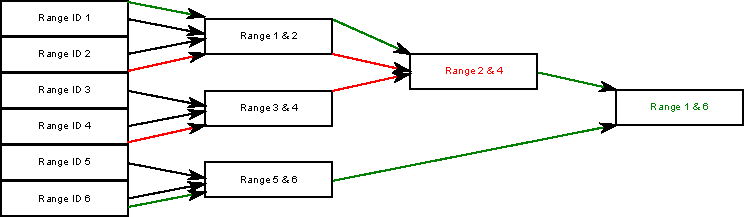
\includegraphics[width=\textwidth]{merging.pdf}
  \caption{Merging Range Objects}
  \label{figure:Merging}
\end{center}
\end{figure}

\begin{figure}[htp]
\begin{center}
  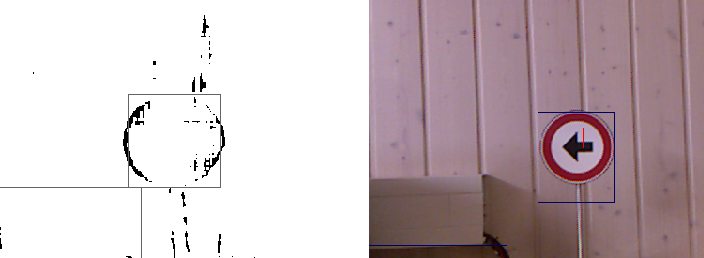
\includegraphics[width=\textwidth]{AnglesOkSegment.png}
  \caption[Angles OK Image and RGB Picture]{Angles OK image and RGB Picture\footnotemark}
  \label{figure:AnglesOKSeg}
\end{center}
\end{figure}
\footnotetext{Camera was held with hands thus pictures are not from the same distance and angle}
\newpage
\begin{lstlisting}[caption={Range Class}\label{lst:RangeClass},language=c++]
class Range
{
	Range *next_range;
	Range *upper1, *upper2;

	std::vector< Range* >* del_vec;

	int x_min;
	int x_max;
	int y_min;
	int y_max;

	cv::Point top_left;
	cv::Point top_right;
	cv::Point bottom_left;
	cv::Point bottom_right;


public:
	Range(int x,int y, std::vector< Range* > *del_vec=NULL)
	: next_range(NULL)
	, upper1(NULL)Surface
	, upper2(NULL)
	, del_vec(del_vec)
	, x_min(x)
	, x_max(x)
	, y_min(y)
	, y_max(y)
	, top_left(x,y)
	, top_right(x,y)
	, bottom_left(x,y)
	, bottom_right(x,y)
	{
		if(del_vec)del_vec->push_back(this);
	}

	Range(const Range &r, std::vector< Range* > *del_vec=NULL)
	: next_range(NULL)
	, upper1(NULL)
	, upper2(NULL)
	, del_vec(del_vec)
	, x_min(r.x_min)
	, x_max(r.x_max)
	, y_min(r.y_min)
	, y_max(r.y_max)
	{
		if(del_vec)del_vec->push_back(this);
	}

	Range(Range *r1, Range *r2)
	: next_range(NULL)
	, upper1(r1)
	, upper2(r2)
	, del_vec(r1->del_vec)
	,x_min((r1->x_min<r2->x_min)?r1->x_min:r2->x_min)
	,x_max((r1->x_max>r2->x_max)?r1->x_max:r2->x_max)
	,y_min((r1->y_min<r2->y_min)?r1->y_min:r2->y_min)
	,y_max((r1->y_max>r2->y_max)?r1->y_max:r2->y_max)
	{
		if(del_vec)del_vec->push_back(this);

		//top_left point
		if((r1->top_left.x+r1->top_left.y)>(r2->top_left.x+r2->top_left.y))
		{
			top_left=r2->top_left;
		}
		else
		{
			top_left=r1->top_left;
		}

		//bottom_right
		if((r1->bottom_right.x+r1->bottom_right.y)<
		   (r2->bottom_right.x+r2->bottom_right.y))
		{
			bottom_right=r2->bottom_right;
		}
		else
		{
			bottom_right=r1->bottom_right;
		}


		//top_right point
		if(x_max-r1->top_right.x+
		   r1->top_right.y<(x_max-r2->top_right.x+r2->top_right.y))
		{
			top_right=r2->top_right;
		}
		else
		{
			top_right=r1->top_right;
		}

		//bottom_left point
		if(x_max-r1->bottom_left.x+
		   r1->bottom_left.y>(x_max-r2->bottom_left.x+r2->bottom_left.y))
		{
			bottom_left=r2->bottom_left;
		}
		else
		{
			bottom_left=r1->bottom_left;
		}
	}

	~Range()
	{
		if(del_vec)return;

		if(upper1!=0)
		{
			upper1->next_range=NULL;
		}
		if(upper2!=0)
		{
			upper2->next_range=NULL;
		}
	}

	void update(int x, int y)
	{
		if(x<x_min)x_min=x;
		if(x>x_max)x_max=x;
		if(y<y_min)y_min=y;
		if(y>y_max)y_max=y;

		//top_left point
		if(top_left.x+top_left.y>(x+y))
		{
			top_left.x=x;
			top_left.y=y;
		}

		//bottom_right
		if(bottom_right.x+bottom_right.y<(x+y))
		{
			bottom_right.x=x;
			bottom_right.y=y;
		}

		//top_right point
		if(x_max-top_right.x+top_right.y<(x_max-x+y))
		{
			top_right.x=x;
			top_right.y=y;
		}

		//bottom_left point
		if(x_max-bottom_left.x+bottom_left.y>(x_max-x+y))
		{
			bottom_left.x=x;
			bottom_left.y=y;
		}
	}

	Range *getLast()
	{
		if(next_range!=NULL)
		{
			return next_range->getLast();
		}
		else
		{
			return this;
		}
	}

	void merge(Range *range)
	{
		Range *r2=range->getLast();
		Range *r1=this->getLast();
		r2->next_range=r1->next_range=new Range(r1,r2);
	}

	Match_Roi getMatchRoi()
	{
		Match_Roi roi;
		roi.top_left=top_left;
		roi.top_right=top_right;
		roi.bottom_left=bottom_left;
		roi.bottom_right=bottom_right;
		roi.roi=cv::Rect(x_min,y_min,x_max-x_min,y_max-y_min);
		return roi;
	}
};
\end{lstlisting}

\begin{lstlisting}[caption={SurfaceExtractor - Function Part 2}\label{lst:SFextract2},language=c++]
	//Merging...
	for(std::set< std::pair<int,int> >::iterator it=relations.begin(); 
	it != relations.end();it++)
	{
		int f=(*it).first-1;
		int s=(*it).second-1;
		ranges[f]->merge(ranges[s]);
	}
	
	std::set<Range*> out;
	for(std::vector<Range*>::iterator it=ranges.begin();it!=ranges.end();it++)
	{
		Range * r=*it;
		r=r->getLast();
		if(out.insert(r).second)//Check if element was inserted
		{
			Match_Roi roi=r->getMatchRoi();
			cv::Rect &cur_rect=roi.roi;
			//Check if rect is inside minimum and maximum size
			if(minHeight<=cur_rect.height && minWidth<=cur_rect.width&&
			   maxHeight>=cur_rect.height && maxWidth>=cur_rect.width)
			rois.push_back(roi);
		}
	}
	for(std::vector<Range*>::iterator it=del_ranges.begin();it!=del_ranges.end();it++)
	{
		delete *it;
	}
}
\end{lstlisting}





\section{RGB Image Processing}

%TODO Perspective ???


If all surface regions have been determined, it's time to start with searching patterns in the
regions. 

\subsection{First template matching approach}
The first approach on finding the signs was done with a HSV color filter and the hough transformation
function from OpenCV, which finds circle in an image or a given region of an image.

The color filter must be in HSV because with that color scheme it is possible to filter for colors
with the H(hue) part of the pixel. In figure \vref{figure:hsv} the green boxes define the color range
which is interesting. Every pixel with another color will be set to zero. The code of that function is
shown in listing \vref{lst:redFilter} and a example picture in figure \vref{figure:redFilter}.

\begin{figure}[htp]
\begin{center}
  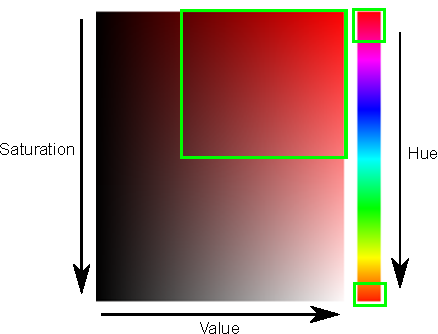
\includegraphics[width=\textwidth]{HSV.pdf}
  \caption{HSV Color Range}
  \label{figure:hsv}
\end{center}
\end{figure}


\begin{figure}[htp]
\begin{center}
  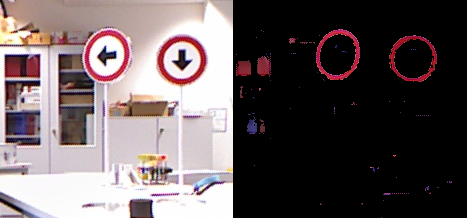
\includegraphics[width=\textwidth]{redFilterResult.png}
  \caption{Result of the HSV based Red Filter}
  \label{figure:redFilter}
\end{center}
\end{figure}


\begin{lstlisting}[caption={RedFilter - Function}\label{lst:redFilter},language=c++]
void RedFilter(const cv::Mat &bgr, cv::Mat &red_out)
{
	cv::Mat hsv;
	red_out=bgr.clone();
	cv::cvtColor( bgr, hsv , CV_RGB2HSV);

	int size_x=bgr.cols, size_y=bgr.rows;
	int y,x;
	for (int i = 0; i < (size_x*size_y); i++)
	{
		//Move forward in vertical direction
		x=i/size_y;
		y=i-x*size_y;

		int h=hsv.at<Vec3uchar>(y,x)[0]*2.83;
		int s=hsv.at<Vec3uchar>(y,x)[1]*0.39;
		int v=hsv.at<Vec3uchar>(y,x)[2]*0.39;


		if(!((h<=13 || h>=338) && s>45 &&v>35))
		{
			red_out.at<Vec3uchar>(y,x)[0]=0;
			red_out.at<Vec3uchar>(y,x)[1]=0;
			red_out.at<Vec3uchar>(y,x)[2]=0;
		}
	}
}
\end{lstlisting}

As seen in the example picture only the circles, some other red objects and some fragments of
other colored objects are visible. The next step is transfering the image to grayscale and 
bluring the image. After that a hugh transformation is executed which will gather round
objects in the picture. If a circle is found a the template is scaled to it's size and 
searched in a region a bit bigger than the found circle.
\newpage
This will most likely bring some good results, but in many cases the inner circle is found
instead of the outer one, and when that happens the image differences are mostly too small
to determine that it is a wrong match(see example in figure \vref{figure:problemCircles}).

\begin{figure}[htp]
\begin{center}
  
\includegraphics[width=\textwidth/2]{robotSignProblem.pdf}
  \caption{Problem with to small circle sizes}
  \label{figure:problemCircles}
\end{center}
\end{figure}

\subsection{Proportion Enhanced Template Matching}
To optimize the template matching another way was found. This algorithm
takes the template picture and converts it to grayscale. It starts at the top left pixel
and searches for the first non translucent pixel diagonally. If it has found one,
it determines if the pixel is dark (value <= 127) or light (value>127). Then it
starts to seek for the next change, when the value passes 127 again.
When it changes the alogrithm gathers the distance from pixel to pixel and searches for the next change.
When that change appears, it calculates the proportion of both lengths.
The proportion will be negative if the next pixels are changing to dark, 
this prevents finding negatives of the template.  
The proportion is stored with the location of the current pixel and the
length of the from the first to the endpoint. This is now done as long
as the algorithm reaches an edge of the template (for an Example see in figure \vref{figure:templateProp}).

\begin{figure}[htp]
\begin{center}
  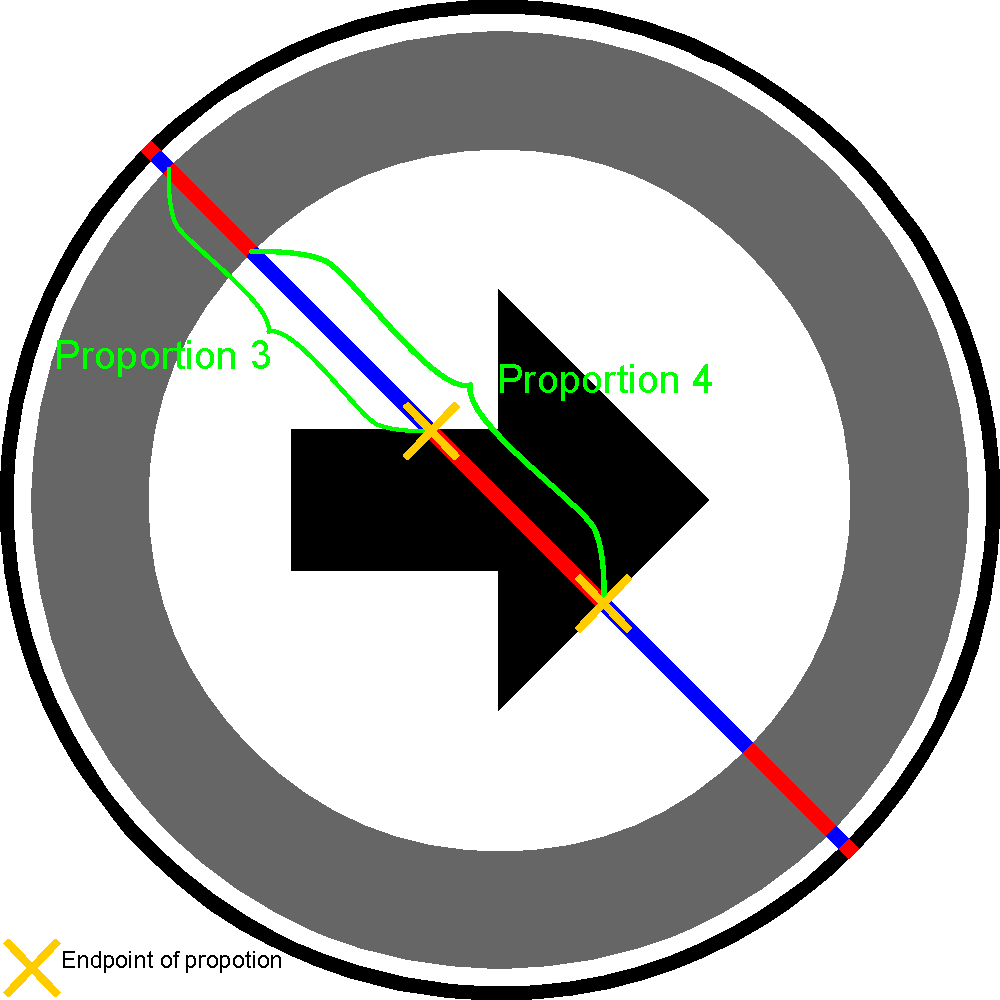
\includegraphics[width=\textwidth/2]{proportionGather.pdf}
  \caption{Gathering Proportions in Template}
  \label{figure:templateProp}
\end{center}
\end{figure}

In the next step the algorithm searches the target picture with the same method, but
it doesn't only search the diagonal row beginning in the top left corner, it searches
through the whole picture. Always when it has two consecutive pixel strings it
creates the proportion. Then it calls a method of the objects the templates are stored in.
This method takes each proportion and checks if this proportion is available for
the current template. If it is, it is stored inside a pair. If a pair of two
consecutive proportions is found it takes the distance length of the last
proportion in the target picture and devides it by the length of the matching proportion
in the template. The resulting factor is used to scale the template to the size of the
proportion in the picture and to determine the new point of the proportion in the scaled template.
With this point the position, for trying to match the template, is calculated 
(see in figure \vref{figure:findPropTempPlace}).

\begin{figure}[htp]
\begin{center}
  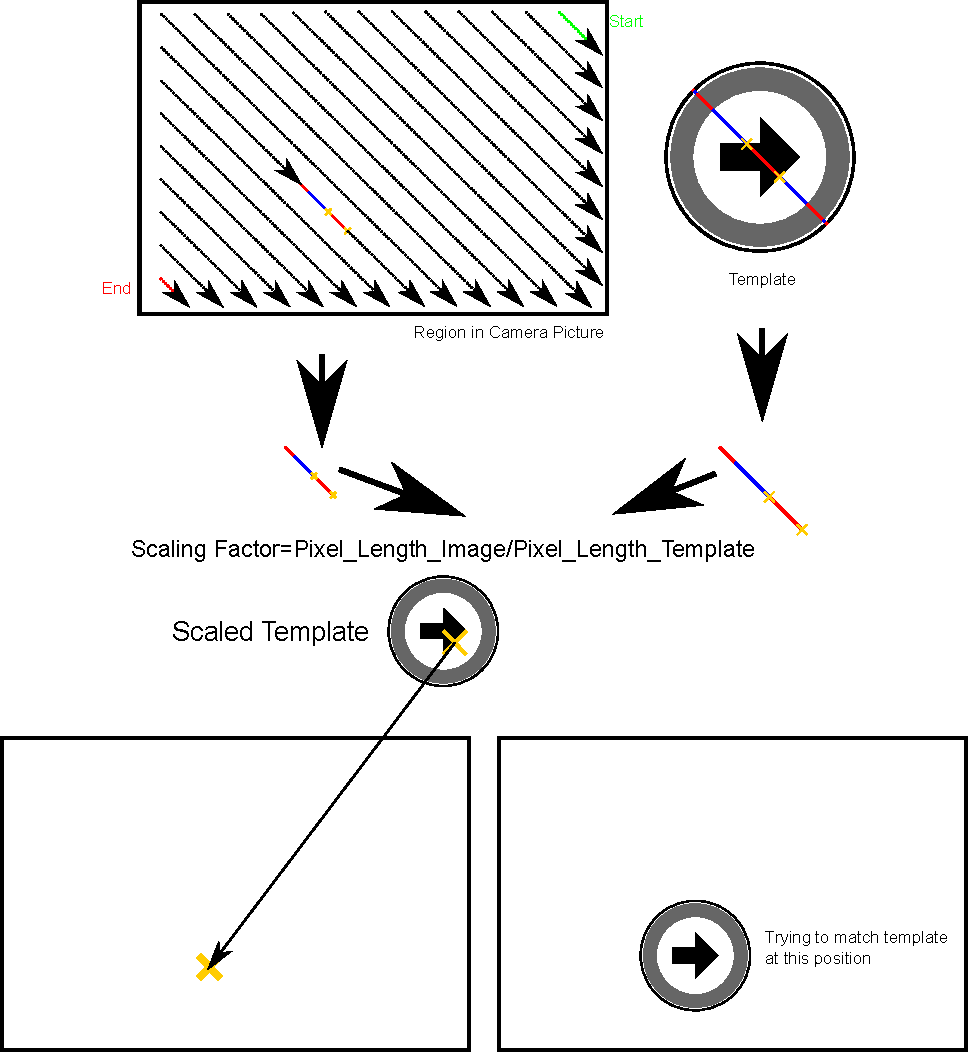
\includegraphics[width=\textwidth]{FindingProportions.pdf}
  \caption{Finding Proportions and Template Placement}
  \label{figure:findPropTempPlace}
\end{center}
\end{figure} 

In the software this is realized by a class called MatchTempProfile in which the templates are stored.
The images for the templates are specified in a xml file which is specified by a parameter in the launchfile.
\newpage 
In the code and the parameter name this file is called settings file. The settings file is read at node startup,
so the code reading the XML file and loading the template pictures is located in the constructor of the
signDetection class seen in listing \vref{lst:ConstructSetTemp}. On startup the node checks first,
if there is a XML file given and if it can be loaded. Then it searches for the "signs"-Tag.
Inside this tag it expects "sign"-Tags with the attributes "name", "file" and "file\_imp".

Listing \vref{lst:xmlFile} shows the XML file used for this project.

The "name" attribut specifies the string which is shown, when this template has been found in a image.
Attribut file specifies the template file which can be a 1,3 or 4 (RGB with alpha channel) channel picture. 
The second image "file\_imp" is optional but expects a grayscale image where important pixels are black and the others 
white. In the special case of a missing or zero size name attribut, the template is called "NONAME" with an increasing number
like "NONAME0, NONAME1 \ldots". If there is no file name specified for the template image or if loading the file
fails, the template profile will not be created. If the file for the important pixel image will fail to load, there will
be just a error message and the profile will be created without an important pixel image. If the paths are relative path 
(beginning with ".." or without "/"), the source path will be the one of the XML file. If everything is ok a new 
MatchTempProfile object (see header contents in figure \vref{lst:MatchTempProfile}) is created and stored in a std::vector.

\begin{lstlisting}[caption={Setting XML File}\label{lst:xmlFile},language=xml]
<?xml version="1.0" ?>
<signs>
<sign name="right"file="../graphics/right.png"file_imp="../graphics/right_imp.png"/>
<sign name="left" file="../graphics/left.png" file_imp="../graphics/left_imp.png"/>
<sign name="stop" file="../graphics/stop.png" file_imp="../graphics/stop_imp.png"/>
</signs>
  
\end{lstlisting}

\newpage
\begin{lstlisting}[caption={signDetection Constructor: Settings File and Templates}\label{lst:ConstructSetTemp},language=c++]
	signDetection() :
	nh_("~"), it_out(nh_)
{
	...
	// Read parameters
	...
	std::string settingsfile;

	nh_.param<std::string>("settingsfile", settingsfile, "");

	if(settingsfile.size())
	{
		ROS_INFO("Settingsfile: %s",settingsfile.c_str());
		TiXmlDocument settings(settingsfile);

		if(settings.LoadFile())
		{
			TiXmlNode *parent, *pChild;

			static int nonames=0;
			//Parsing the XML
			parent=settings.FirstChildElement();

			//Reading the settingsfile
			for ( pChild = parent->FirstChild(); pChild != 0; 
			      pChild = pChild->NextSibling())
			{
				//Look for Elements
				if(pChild->Type()==TiXmlNode::TINYXML_ELEMENT)
				{
					TiXmlElement* pElement=pChild->ToElement();
					if(pElement->ValueStr()=="sign")//If the element is sign
					{
						TiXmlAttribute* pAttrib=pElement->FirstAttribute();
						bool imgloaded=false;
						printf("\n");
						std::string name;
						std::string file;
						std::string file_imp;
						while (pAttrib) //fetch attributes
						{
							if(pAttrib->NameTStr()=="name") //sign name
							{
								name=pAttrib->Value();
							}
							if(pAttrib->NameTStr()=="file") //file name
							{
								file=pAttrib->Value();
							}
							if(pAttrib->NameTStr()=="file_imp") //file name (important pixels)
							{
								file_imp=pAttrib->Value();
							}

							pAttrib=pAttrib->Next();
						}


						if(!name.size())//if no name tag is specified create a noname
						{
							std::stringstream ss;
							ss<<"NONAME_"<<nonames;
							name=ss.str();
							nonames++;
						}

						if(file.size())//Is there a filestring for template picture
						{
							boost::filesystem::path picturePath(file);
							if(picturePath.is_relative())//Is it a relative path?
							{
								boost::filesystem::path xmlfilepath(settingsfile);
								boost::filesystem::path xmldir=xmlfilepath.parent_path();
								picturePath=xmldir/=picturePath;
							}

							//Is there a file for important pixels?
							boost::filesystem::path picturePath2(file_imp);
							if(picturePath2.is_relative()) //Is it a relative path?
							{
								boost::filesystem::path xmlfilepath(settingsfile);
								boost::filesystem::path xmldir=xmlfilepath.parent_path();
								picturePath2=xmldir/=picturePath2;
							}

							ROS_INFO("File: %s", picturePath.string().c_str());
							cv::Mat img=cv::imread(picturePath.string());
							cv::Mat img_imp=cv::imread(picturePath2.string());
							if(!img.empty())
							{
								if(!img_imp.empty())
								{
									ROS_INFO("Loaded img_imp: %s",file_imp.c_str());
									tempProfiles.push_back(
									KinTo::MatchTempProfile
									(img,img_imp,name,0.08,0.2,127,0.2,0.7,0.8));
								}
								else
								{
									tempProfiles.push_back(
									KinTo::MatchTempProfile
									(img,name,0.08,0.2,127,0.2,0.7,0.8));
									if(file_imp.size())
									{
										ROS_ERROR("Could not load given imp_file: "
										"%s, going on without it...",file_imp.c_str());
									}
								}

								signs.push_back(sign(name,img));
								imgloaded=true;
							}
						}
						else
						{
							imgloaded=false;
						}

						if(imgloaded)
						{
							ROS_INFO("New Sign: %s",name.c_str());
						}
						else
						{
							ROS_INFO("Sign: %s, Could not be loaded!",name.c_str());
						}
					}
				}
			}
		}
		else
		{
			ROS_ERROR("Could not load settings file: %s", settingsfile.c_str());
		}
	}
	else
	{
		ROS_ERROR("NO SETTINGS FILE GIVEN!!!");
	}
	...

}
\end{lstlisting}



\begin{lstlisting}[caption={MatchTempProfile (Header)}\label{lst:MatchTempProfile},language=c++]
class MatchTempProfile
{
public:

	typedef std::pair<Proportion, Proportion> proportion_pair;

private:
	std::vector<Match> matches;
	std::vector<Proportion> proportions;
	cv::Mat tmp, gray;
	cv::Point begin, end;
	proportion_pair last_pair;
	double max_proportion_diff;
	double min_congruence;
	double min_coverage;
	std::string name;
	double min_target_size;
	double max_target_size;
	cv::Mat important_pixels;
	bool hasImportantPixels;

	void constructor_extension(int threshold);
	void templateMatching(Proportion fromTemplate,  
	                      Proportion fromTarget,
	                      const cv::Mat& target,
	                      int threshold);
public:
	MatchTempProfile(const cv::Mat &tmp, std::string name, 
	                 double minimal_target_size=.1, 
	                 double max_target_size=0.25, 
	                 uchar threshold=127, 
	                 double max_proportion_diff=0.4, 
	                 double min_coverage=0.6, 
	                 double min_congruence=0.7);

	MatchTempProfile(const cv::Mat &tmp, 
					const cv::Mat &tmp_imp, 
					std::string name, 
					double minimal_target_size=.1, 
					double max_target_size=0.25, 
					uchar threshold=127, 
					double max_proportion_diff=0.4, 
					double min_coverage=0.6, 
					double min_congruence=0.8);

	void checkProportion(Proportion proportion, 
						const cv::Mat &target, 
						int threshold=127);

	void reset_ProportionCheck();

	const std::vector<Match>& getMatches()
	{
		return matches;
	}

	void clearMatches()
	{
		matches.clear();
	}
};
\end{lstlisting}


Later when there is a image or region of interest, where to search for the template, the function
proportionEnhancedTemplateMatching (see source in listing \vref{lst:propEnhTM}) is called with the vector 
of the MatchTempProfile objects and the target image/region as parameters. This function 
scans the image as mentioned above and everytime it finds two dark/light changes, it creates a proportion
object (see Source in listing \vref{lst:proportion}) and hands it to the checkProportion function
(shown in listing \vref{lst:checkProportion}) in each MatchTempProfile inside the array.
This function stores the current value into the second variable of a pair and sets the first to
the second variable before. If it has two values for one pair it seeks  
for this pair in the proportion array. If it finds a suitable pair of proportions (inside the given threshold) 
it calls the function templateMatching of the MatchTempProfile object (see source in listing \vref{lst:templateMatching}).
This function does the scaling of the template and the recalculation of the point and after this,
it tries to match the template against the relevant region. Calculating the new point is
done by multiplying both x and y coordinates with the scaling factor. The matching is done like
the gathering of the proportions. Values are checked if they are both dark or light, if that
is the case, the counter for equal pixels is increased by one. If a picture for important pixels
is available a counter is increased if pixels on a important location do not match. For all compared
pixels another counter is increased to determine the coverage factor of the pattern.

In the end the following quotients are calculated:
$$
	\mbox{congruence} =\frac{\mbox{matching pixels}}{\mbox{compared pixels}}-\frac{\mbox{non-matching important pixels}}{2}
$$
$$
	\mbox{coverage} = \frac{\mbox{compared pixels}}{\mbox{pixel count of template}}
$$

If the quotients are in the specified range which are given at the template creation, the results 
are stored in form of a Match object inside a vector in the corresponding MatchTempProfile object.

If all proportions of a region are checked for the current surface, the best matching template will
be marked in the picture with the first letter of it's name. And then the arrays,
which hold the Match objects for each profile, are cleared for the next region.

This is the reason why the application only supports \textbf{one sign per surface} at the moment.

An example result to this algorithm can be seen in figure \vref{figure:MatchingSigns}.

\newpage
\begin{lstlisting}[caption={proportionEnhancedTemplateMatching}\label{lst:propEnhTM},language=c++]
void proportionEnhancedTemplateMatching(std::vector<MatchTempProfile> 
                                        &templates, const cv::Mat &target, 
                                        uchar threshold)
{

	cv::Mat blured;
	cv::cvtColor(target, blured, CV_BGR2GRAY);
	cv::equalizeHist(blured,blured);

	cv::GaussianBlur(blured,blured,cv::Size(5,5),2,2,0);




	int size_x=target.cols;
	int size_y=target.rows;

	int x_dia=size_x-1;
	int y_dia=0;

	int start_col=size_x-1;
	int start_row=0;

	int last_length=-1;
	int current_length=0;
	int dark=0;

	for(int i=0; i<(size_x*size_y);i++)
	{


		if(y_dia>=size_y || x_dia>=size_x)
		{
			if(start_col>0)
			{
				start_col--;
				x_dia=start_col;
				y_dia=0;
			}
			else
			{
				start_row++;
				x_dia=0;
				y_dia=start_row;
			}
		}
		///////////////////////////////////////////////////////
		////////////////////////////////DIAGONAL X/Y///////////
		if(y_dia == 0 || x_dia==0)
		{
			dark=blured.at<Vec1uchar>(y_dia,x_dia)[0]<threshold;
			last_length=-1;
			current_length=0;
			for(std::vector<MatchTempProfile>::iterator it=templates.begin();
										it!=templates.end();
										it++)
			{
				it->reset_ProportionCheck();
			}
		}

		bool current=blured.at<Vec1uchar>(y_dia,x_dia)[0]<threshold;

		if(dark != current)
		{
			dark=current;
			if(last_length!=-1)
			{
				Proportion prop;
				prop.length_c=current_length;
				prop.length_l=last_length;
				prop.proportion=(1-2*dark)*(double)last_length/(double)current_length;
				prop.x=x_dia;
				prop.y=y_dia;

				for(std::vector<MatchTempProfile>::iterator it=templates.begin();
								it!=templates.end();
								it++)
				{
					it->checkProportion(prop,blured,127);
				}
			}
			last_length=current_length;
			current_length=0;

		}
		current_length++;


		///////////////////////////////////////////////////////////
		///////////////////////////////////////////////////////////
		x_dia++;
		y_dia++;
	}
}
\end{lstlisting}

\newpage
\begin{lstlisting}[caption={Proportion Class}\label{lst:proportion},language=c++]
	class Proportion
	{
	public:
		double proportion;
		int x;
		int y;
		int length_l;
		int length_c;
	
		Proportion()
		:proportion(-1)
		,x(-1)
		,y(-1)
		,length_l(-1)
		,length_c(-1)
		{}
	};
\end{lstlisting}

\newpage
\begin{lstlisting}[caption={MatchTempProfile::checkProportion - Function}\label{lst:checkProportion},language=c++]
void MatchTempProfile::checkProportion(Proportion proportion, 
                          const cv::Mat &target, int threshold)
{
	//Move second to first
	last_pair.first=last_pair.second;
	//Save current to second
	last_pair.second=proportion;

	//If it already contains a pair
	if(last_pair.first.proportion!=-1)
	{
		//Seek for pair in proportions
		for(std::vector<Proportion>::iterator it=proportions.begin()
				;it!=proportions.end();it++)
		{
			Proportion *p1=&(*it);
			if(std::fabs(p1->proportion-last_pair.first.proportion)<=max_proportion_diff)
			{
				if(it+1 != proportions.end())
				{
					Proportion *p2=&(*(it+1));
					if(std::fabs(p2->proportion-last_pair.second.proportion)
					   <=max_proportion_diff)
					{
						templateMatching(*(it+1), proportion, target, threshold);
					}
				}
			}
		}
	}
}
\end{lstlisting}

\newpage
\begin{lstlisting}[caption={MatchTempProfile::templateMatching - Function}\label{lst:templateMatching},language=c++]
void MatchTempProfile::templateMatching(Proportion fromTemplate, 
                                        Proportion fromTarget,
                                        const cv::Mat& target,
                                        int threshold)
{

	//scaling factor for the template
	double scaling_factor=(double)fromTarget.length_l+(double)fromTarget.length_c;
	scaling_factor/=(double)fromTemplate.length_c+(double)fromTemplate.length_l;

	if(scaling_factor<=0)
	{
		std::cerr<<"MatchTemplateProfile::templateMatching "
		           "scaling_factor smaller or equal zero"<<std::endl;
		return;
	}


	if(scaling_factor<min_target_size || scaling_factor>max_target_size)return;

	//scale the template picture
	cv::Mat scaled_template, scaled_imp_template;
	cv::resize(gray,scaled_template,cv::Size(0,0),scaling_factor,scaling_factor);

	if(!important_pixels.empty())
	{
		cv::resize(important_pixels,scaled_imp_template,
		           cv::Size(0,0),scaling_factor,scaling_factor);
	}



	//recalculate the point of the proportion
	int x_st=fromTemplate.x*scaling_factor;
	int y_st=fromTemplate.y*scaling_factor;

	//calculate the point for template placement
	int x_tplace=fromTarget.x-x_st;
	int y_tplace=fromTarget.y-y_st;

	int size_x=scaled_template.cols;
	int size_y=scaled_template.rows;

	cv::Rect r;
	r.height=scaled_template.rows;
	r.width=scaled_template.cols;
	r.x=x_tplace;
	r.y=y_tplace;


	int cnt_pixelsCmp=0;
	int cnt_pixelsOk=0;
	int cnt_pixelsNegative=0;



	for(int i=0; i<(size_x*size_y);i++)
	{
		int y_temp=i/size_x;
		int x_temp=i-y_temp*size_x;

		int x_targ=x_temp+x_tplace;
		int y_targ=y_temp+y_tplace;



		if(x_targ>=0 && x_targ<target.cols &&
		   y_targ>=0 && y_targ<target.rows )
		{
			//TODO ignore translucent pixels
			cnt_pixelsCmp++;

			bool val_tmp=scaled_template.at<Vec1uchar>(y_temp,x_temp)[0]>127;
			bool val_trg=target.at<Vec1uchar>(y_targ,x_targ)[0]>127;


			if(val_tmp==val_trg)
			{
				cnt_pixelsOk++;
			}
			else
			{
				if(hasImportantPixels)
				{
					if(scaled_imp_template.at<Vec1uchar>(y_temp,x_temp)[0]==0)
					{
						cnt_pixelsNegative++;
					}
				}
			}
		}
	}
	

	double congruence=(double)cnt_pixelsOk/(double)cnt_pixelsCmp-cnt_pixelsNegative/2;
	double coverage=(double)cnt_pixelsCmp/(double)(size_x*size_y);

	if(congruence>=min_congruence && coverage>=min_coverage)
	{
		Match m;
		m.congruence=congruence;
		m.coverage=coverage;
		m.rect.x=x_tplace;
		m.rect.y=y_tplace;
		m.rect.width=size_x;
		m.rect.height=size_y;
		m.center=cv::Point(x_tplace+size_x/2, y_tplace+size_y/2);
		m.name=name;

		matches.push_back(m);
	}
}
\end{lstlisting}



\section{Robot Control}
\subsection{ROS Transform}
\subsection{Navigation}
